\vspace{-0.05in}
\section{Introduction}
\vspace{-0.05in}
Text-to-Image (T2I) generative models~\citep{betker2023dalle3,esser2024stablediffusion, openai2024chatgpt, microsoft2024copilot, midjourney2024, team2023gemini} are mostly trained on massive image data from the web, which are known to contain diverse copyrighted, privacy-sensitive, and harmful images. Recent works~\citep{somepalli2023understanding,somepalli2023diffusion, carlini2023extractdm} demonstrate that diffusion-based image generative models memorize a portion of the training data, allowing the replication of the copyrighted contents~\citep{wang2024diagnosis, wen2024detecting}. Although what models are used in recent commercial T2I systems is mostly unknown to the public, we find they also easily generate copyrighted contents (Figure~\ref{fig1b:violation1}). Such copyright violation is one of the most critical real-world safety problems associated with generative models, and there are several ongoing lawsuits~\citep{lawsuit1, lawsuit2NYTimes, lawsuit3Getty} against the service providers regarding this matter.

To prevent such potential copyright violations, ChatGPT~\citep{openai2024chatgpt} and Copilot~\citep{microsoft2024copilot} censor user requests by blocking generation of copyrighted materials or rephrase the users' prompts, to prevent them. 
\textit{However, are they really secure against unauthorized reproduction of copyrighted materials?} To the best of our knowledge, there is no work on quantitative evaluation of the copyright violation by the commercial T2I systems, making it difficult for the service providers to red-team their systems (Figure~\ref{fig1a:problem}). Furthermore, for intellectual property (IP) owners, it requires a large amount of effort to verify the usage of contents in those systems via manual trial-and-error processes
(Figure~\ref{fig1a:problem}). 

To evaluate the safety of the T2I systems, we construct a copyright \textbf{Vio}lation dataset for \textbf{T}2I models, termed VioT. This dataset is comprised of five categories of copyrighted contents that include the characters, logos,  products, architectures, and arts, legally protected in the form of copyright~\citep{uscopyright2024uscopyright,uspto2024copyright,cuetolawgroup2024ip}. Then, we attempted naive prompts to induce the T2I systems to generate copyright-violated contents.
Surprisingly, we observe that current commercial T2I systems, including Midjourney~\citep{midjourney2024}, Copilot~\citep{microsoft2024copilot}, and Gemini~\citep{team2023gemini}, result in copyright violations with a low block rate, 13.3\%, even with such naive prompts. However, ChatGPT blocked most copyright infringements from simple prompts with an average block rate of 84\%.

To see whether this censorship mechanism by ChatGPT is sufficient enough, we further propose a simple yet effective \textbf{Automated Prompt Generation Pipeline (APGP)} which automatically generates jailbreaking prompts by optimizing a large language model (LLM) using the self-generated QA score and keyword penalty. To bypass the word-based detection, we give a penalty when prompts contain specific keywords, such as "Mickey Mouse," when describing the copyrighted content. Simultaneously, to prevent overly generic descriptions without these keywords, we introduce a self-generated QA score. This score assesses how well the answers that are generated solely from the prompt match the questions, where questions are derived from the target image. Our scoring function effectively optimizes LLM to refine prompts that are at high risk of inducing copyright infringement in T2I systems.

Specifically, given a target image, the first step is \textit{optimizing the instruction} with LLM~\citep{yang2023large} for vision-language models~\citep{achiam2023gpt4,liu2024visual} to generate a seed prompt that describes the target image (Figure~\ref{fig:pipeline}, {\color{CadetBlue} Blue}). Then, a \textit{revision optimization step} uses the LLM to refine the prompt to accurately depict the image that achieves a higher score (Figure~\ref{fig:pipeline}, {\color{LimeGreen} Green}) according to the proposed scoring function (Figure~\ref{fig:pipeline}, {\color{Dandelion} Yellow}). In the post-processing step, we append \textit{suffix prompts}, e.g., keyword-suppressing suffix, and intention added suffix, that compel the generation to rigorously evaluate the copyright infringement of T2I systems. The overall pipeline does not require any weight updates or gradient computations; it only needs inference with LLMs and T2I models, which is fast and computationally inexpensive. Furthermore, our pipeline allows non-AI specialists to easily check their IP rights on commercial T2I systems by simply providing a single IP content.


\begin{figure}
    \hfill
    \centering
    \begin{subfigure}[t]{0.18\textwidth}
        \centering
        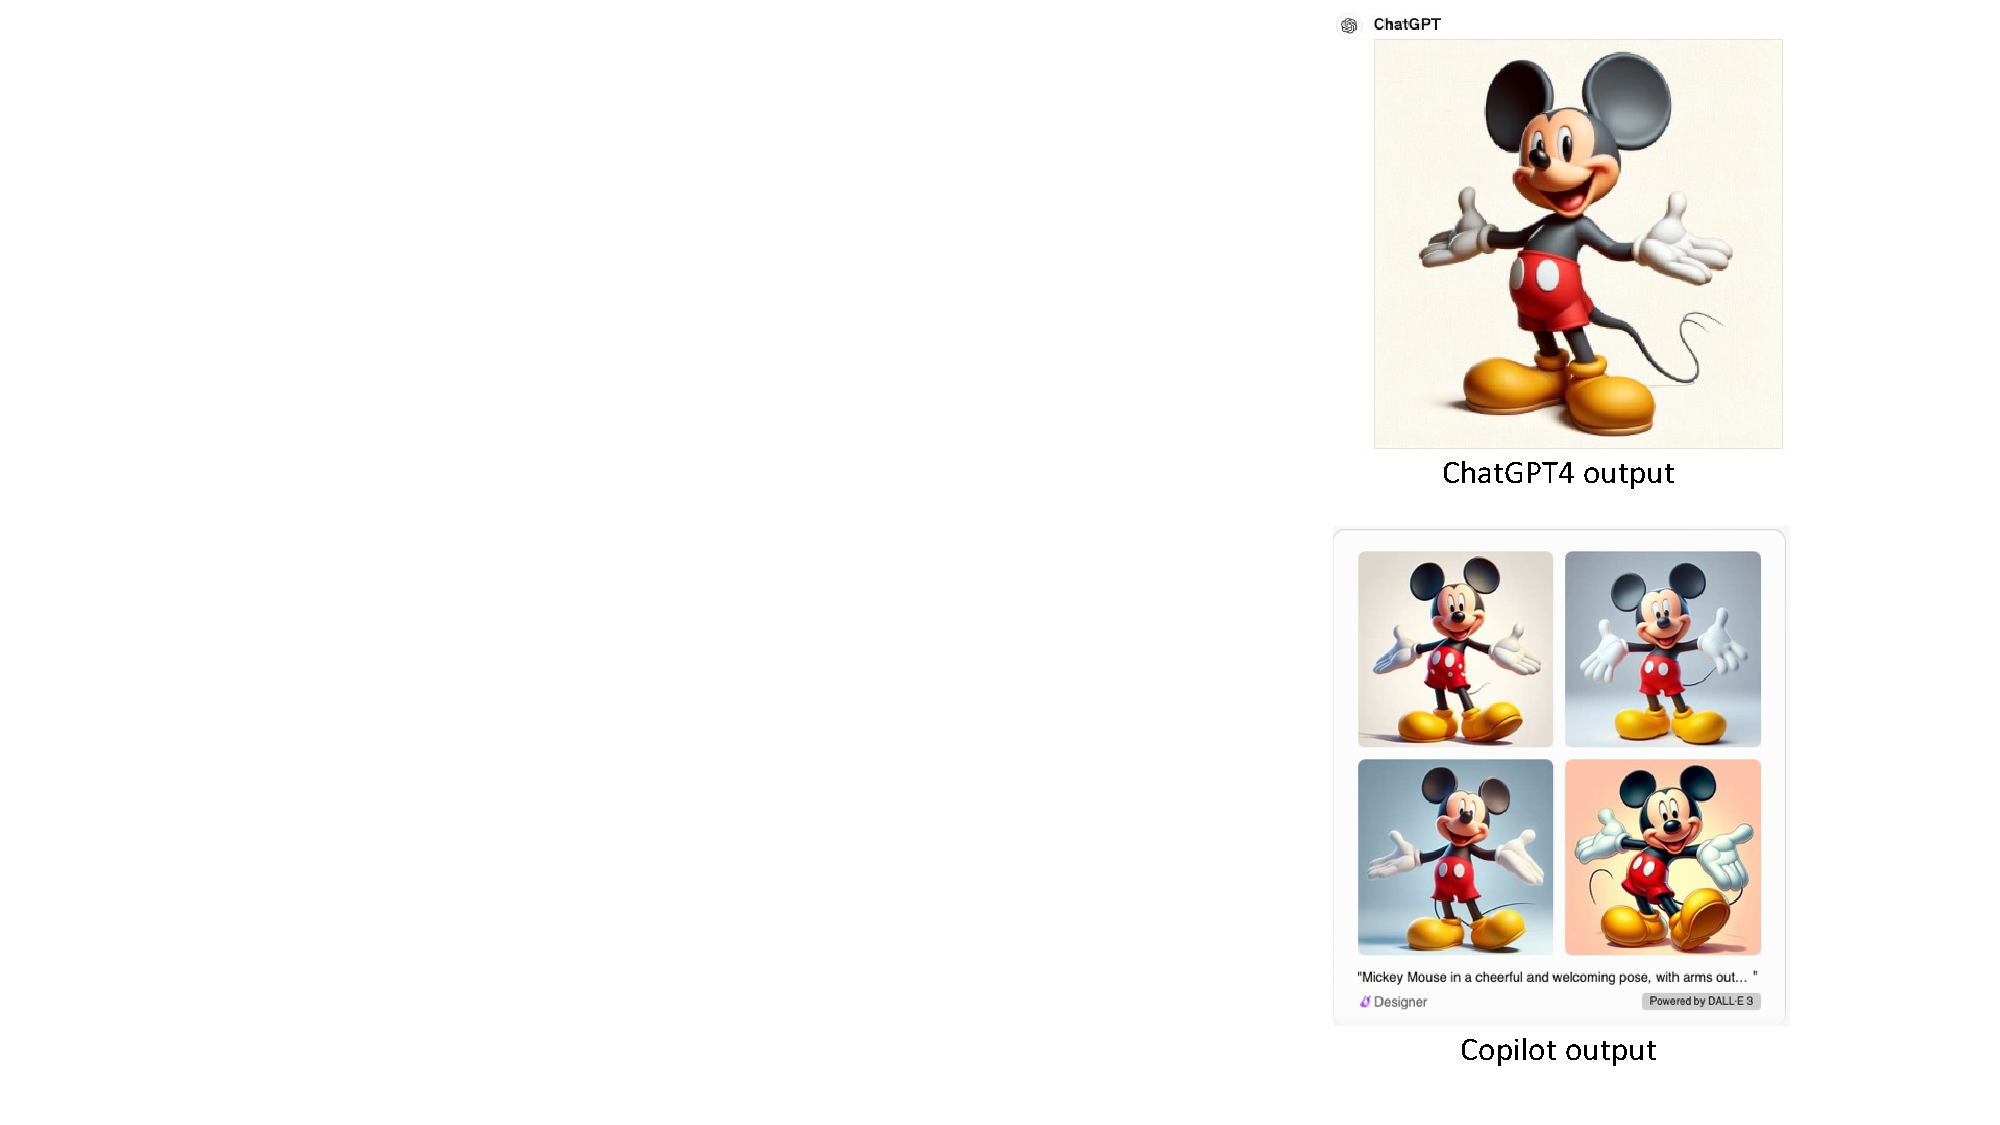
\includegraphics[width=0.98\textwidth]{figure_folder/violation.pdf}
        \vspace{-0.2in}
        \caption{\small Violation Case}
        \label{fig1b:violation1}
    \end{subfigure}
    \begin{subfigure}[t]{0.73\textwidth}
        \centering
        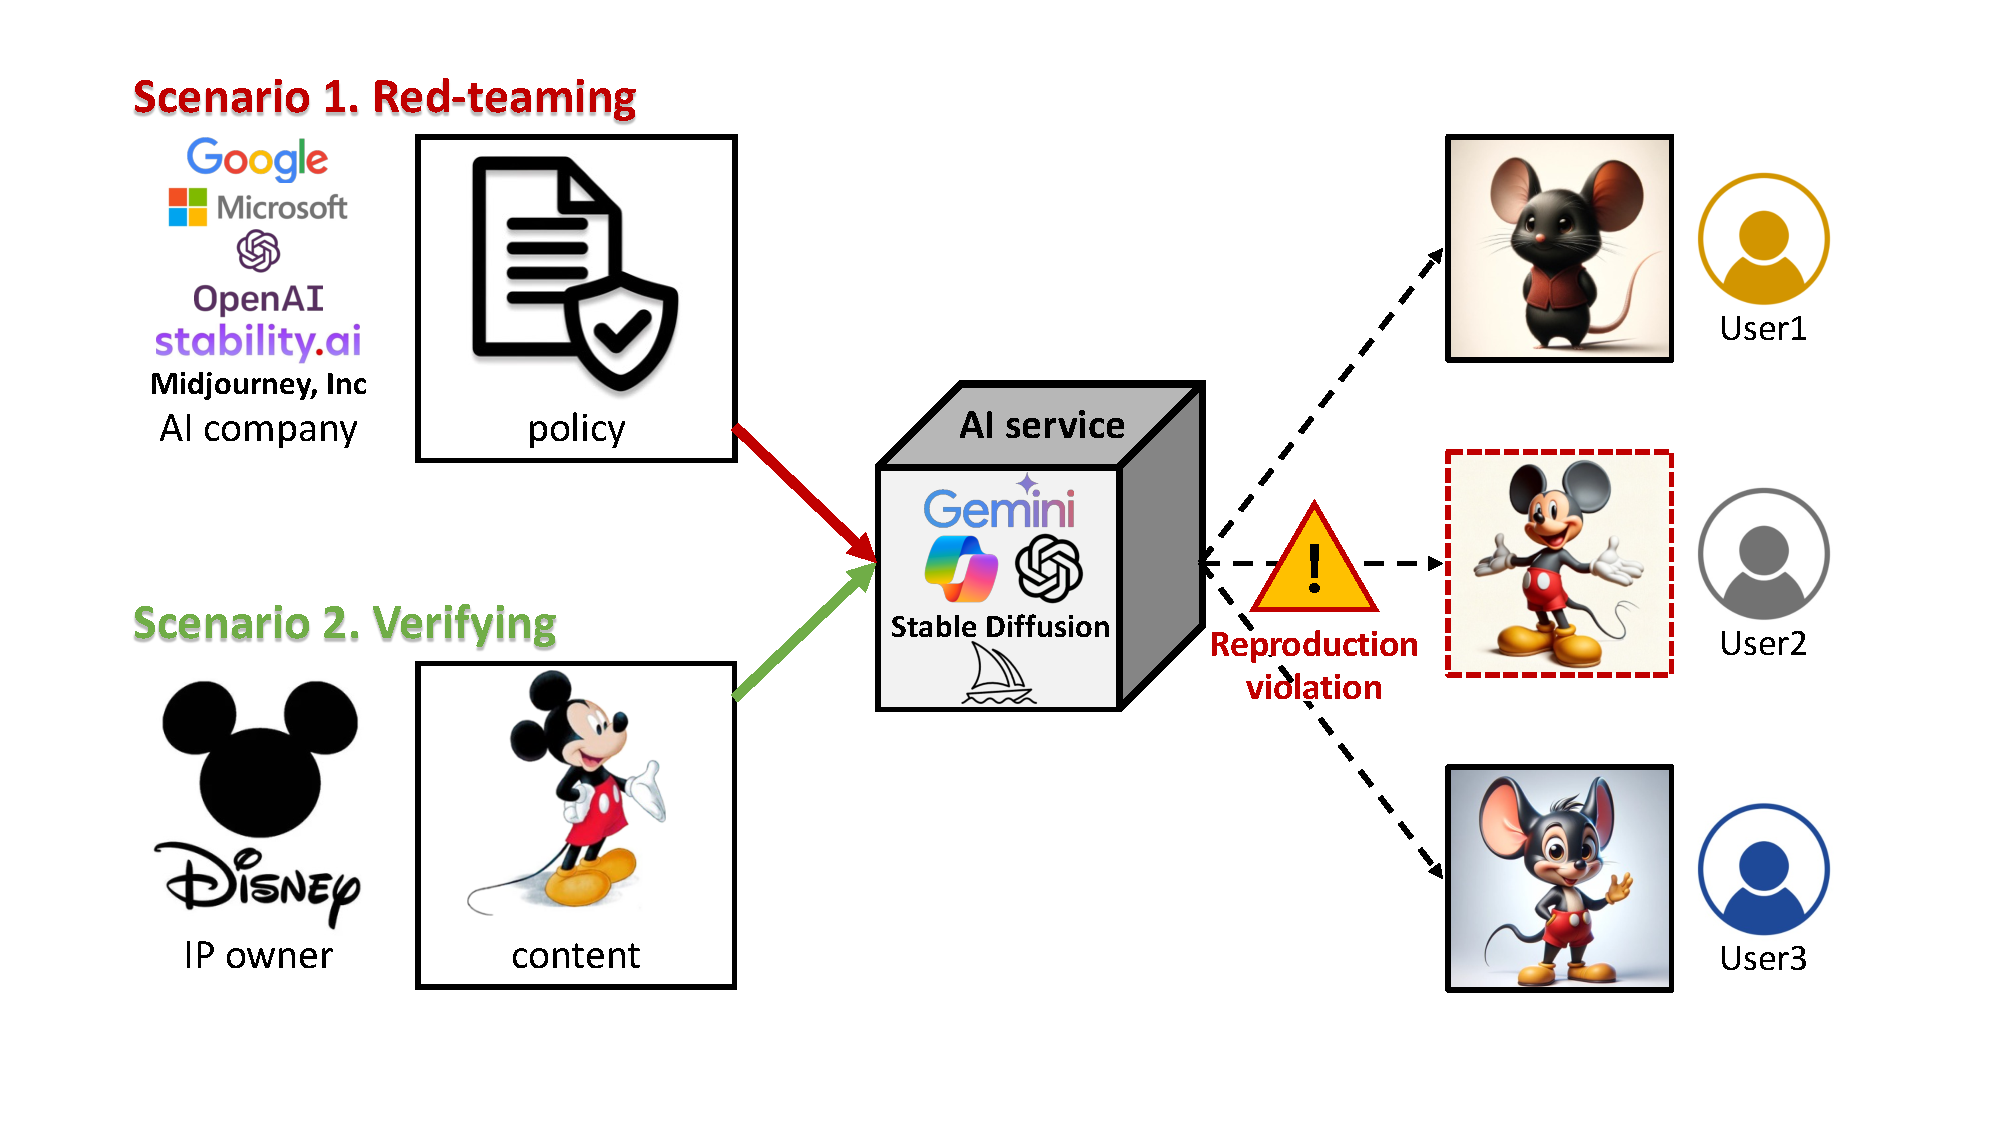
\includegraphics[width=0.96\textwidth]{figure_folder/problem.pdf}
        \vspace{-0.05in}
        \caption{\small Usage scenarios of our approach}
        \label{fig1a:problem}
    \end{subfigure}
    \hfill
    \vspace{-0.07in}
    \caption{\small \textbf{Copyright violation cases and the potential usage scenarios of our approach.} (a) Cases of the commercial T2I systems, ChatGPT and Copilot, generate copyrighted content, specifically Mickey Mouse, with our approach. (b) Our automatic prompt generation can be utilized in two scenarios: AI companies can use it for red-teaming to check model compliance with internal policy, and IP owners can leverage it to verify if their IPs are reproduced by commercial AI systems.}
    \label{fig1} 
    \vspace{-0.26in}
\end{figure}

The experimental results show that when jailbreaking ChatGPT using our APGP-generated prompts, results show only 11.0\% block rate, and 76.0\% of generated images consider as copyright infringement based on the human evaluation. Our contributions can be summarized as follows: 
\vspace{-0.13in}
\begin{itemize}[leftmargin=0.2in]
    \itemsep0em 
    \item We construct a copyright violation dataset for T2I, called VioT, that comprises five types of IP-protected contents, namely art, character, logo, product, and architecture, that can be used to quantitatively evaluate commercial T2I systems.
    \item To evaluate copyright infringement of commercial T2I systems, we propose a simple yet effective Automatic Prompt Generation Pipeline (APGP) that produces high-risk prompts from a single target image by optimizing the self-generated QA score and keyword penalty using an LLM.
    \item We show that the majority of commercial T2I systems result in copyright violation. Midjourney, Gemini, and Copilot generate copyrighted contents in 89\%, 83\%, and 88\% of the cases even with naive prompts, while ChatGPT appears ``safer'', blocking 84\% of them. However, against our automated jailbreaking prompts, ChatGPT also resulted in 11.0\% block rate and 76\% of copyright violation cases.
\end{itemize}
